\chapter{Nutzungskontext}
Bei der Analyse des Nutzungskontextes wird zunächst auf die beteiligten Personen und Gruppen eingegangen um anschließend zu untersuchen, mit welchen Erwartungen sie in welchen Szenarien an die Anwendung herantreten.

\subsubsection*{Anwender(Akteure)}
\begin{itemize}
  \item Studenten
  \item Mitarbeiter der FH Koeln (extern/intern)
  \item Besucher/Fremde
\end{itemize}

\noindent
Die Anwender lassen sich allerdings auch auf andere Kategorien aufteilen, welche ihre für die Anwendung relevanten Eigenschaften besser abbilden.
\begin{itemize}
  \item Junge/Gesunde Menschen
  \item Alte Menschen
  \item Menschen mit und ohne Deutschkenntnisse
  \item Kranke/Verletzte Menschen
  \item Sehbehinderte Menschen
  \item Rollstuhlfahrer
\end{itemize}

\noindent
Ein wesentlicher Punkt ist das sich die verschiedenen Kategorien überlappen, es könnte beispielsweise ein Rollstuhlfahrer mit eingeschränkten Deutschkenntnissen den Wunsch haben, sich in der Fachhochschule navigieren zu lassen.

\subsubsection*{Stakeholder}
\begin{itemize}
  \item Dozenten/Auftraggeber
  \item Am Projekt beteiligte Studenten
\end{itemize}

\subsubsection*{Mentale Modelle}
Ein weiteres wichtiges Werkzeug in der Mensch-\-Computer-\-Interaktion ist der Einsatz von \emph{mentalen Modellen}, welche die Erwartungen und den internen Zustand des Nutzers bei der Bedienung der Anwendung beschreiben. \medskip

\noindent Der User erwartet...
\begin{itemize}
  \item dass die Navigationsanwendung ihn Schritt für Schritt an sein Ziel führt und ihm visuell und akustisch mitteilt wie er ans Ziel gelangt bzw. wie er seinen nächsten Schritt macht
  \item \textbf{nicht}, dass er sein Ziel anhand eines abgebildeten Weges auf einer 2D-Karte finden muss
  \item dass er auf Hindernisse auf seiner Zielroute hingewiesen wird und bei einer Blockade eine alternative Route geliefert bekommt
  \item dass er Orte auch nach Bezeichnungen oder ihrem Zweck suchen kann (Mensa, WC, \dots)
\end{itemize}

\subsubsection*{Persona}
Personas stellen Prototypen für Gruppen von Nutzern mit konkret ausgeprägten Eigenschaften und einem konkreten Nutzungsverhalten dar. Sie werden genutzt um User-Stories zu definieren.

\begin{itemize}
  \item \textbf{Max Mustertyp (25)}, Informatikstudent im 4. Semester, keine physischen Einschränkungen
  \item \textbf{Hans Herd (64)}, Firmenvertreter, Besucher an der FH, Rollstuhlfahrer
  \item \textbf{Hannes Pannes (20)}, Ingenieurwissenschaftenstudent, vor kurzem ein Bein gebrochen
  \item \textbf{Peter Meter (44)}, Dozent an der FH, Blind
  \item \textbf{Ali Mali(26)}, Informatik-austauschstudent, hat sehr eingeschränkte deutsche Sprachkenntnisse
  \item \textbf{Jürgen Würgen (44)}, externer Elektriker, nutzt einen Werkzeugwagen 
\end{itemize}

\subsubsection*{User-Stories}
\begin{itemize}
\item Als FH-Besucher möchte ich mein Profil festlegen, um trotz meinen ggf. körperlichen Einschränkungen ans einen Zielort gelangen zu können.
\item Als FH-Besucher möchte ich Wegoptionen wählen können, um unabhängig von meinem festgelegten Profil alternative Routen wählen zu können. (Beispiel: User ist faul oder temporär physich eingeschränkt)
\item Als FH-Besucher möchte ich einen Zielort wählen können, um auch unabhängig von Raumnummern an einen Ort gelangen zu können.
\item Als FH-Besucher möchte ich auch dann ans Ziel gelangen, wenn mir die Raumnummer nicht bekannt ist, dazu möchte ich ein Anliegen auswählen.
\item Als FH-Besucher mit entsprechendem Profil möchte ich meine Anliegen statt von Hand auch per Spracheingabe eingeben können
\end{itemize}

\subsubsection*{Szenarien}
\begin{enumerate}
  \item Max Mustertyp hat heute IM-Praktikum, das Praktikum findet in R1234 statt, er hat die Raumnummer im Stundenplan nachgeschaut und möchte sich nun bequem dorthin navigieren lassen. Max startet nun die Navigationsanwendung auf seinem Smartphone und tippt die Raumnummer ein. Nun startet er die Navigation.
  \item Peter Meter muss gleich eine Vorlesung halten, das Semester hat gerade erst begonnen und seine Vorlesung findet nun in einem anderen, ihm nicht gewohnten Raum statt. Um den Raum zu finden möchte er die Navigationsanwendung auf seinem Smartphone nutzen. Er startet also die Navigations-App und nennt die Raumnummer, welche via Spracheingabe erfasst wird. Mit den Worten “Navigation jetzt starten”, wird er nun per Sprachausgabe an sein Ziel geführt.
  \item Jürgen Würgen hat den Auftrag einige Lampen im dritten Stock zu tauschen, er war noch nie am Campus Gummersbach und weiß deshalb nicht wo es lang geht. Er fährt auf den Parkplatz des Campus, geht durch den Haupteingang hinein und stellt fest, dass er mit seinem schweren Werkzeugwagen nicht die Treppen hinauf kommt. Um eine alternative Route zu finden, startet er die Navigationsapp und trägt den ersten der ihm genannten Räume ein. Um nicht die Treppen nutzen zu müssen, verbietet er in den Wegoptionen die Treppen.
\end{enumerate}

\subsubsection*{Use Case Diagramm (Verhalten)}
... bietet eine standardisierte Möglichkeit um die zuvor genannten Nutzer und ihre Use Cases sowie die Beziehungen zwischen Use Cases untereinander darzustellen.

\begin{figure}[hbt]
  \centering
  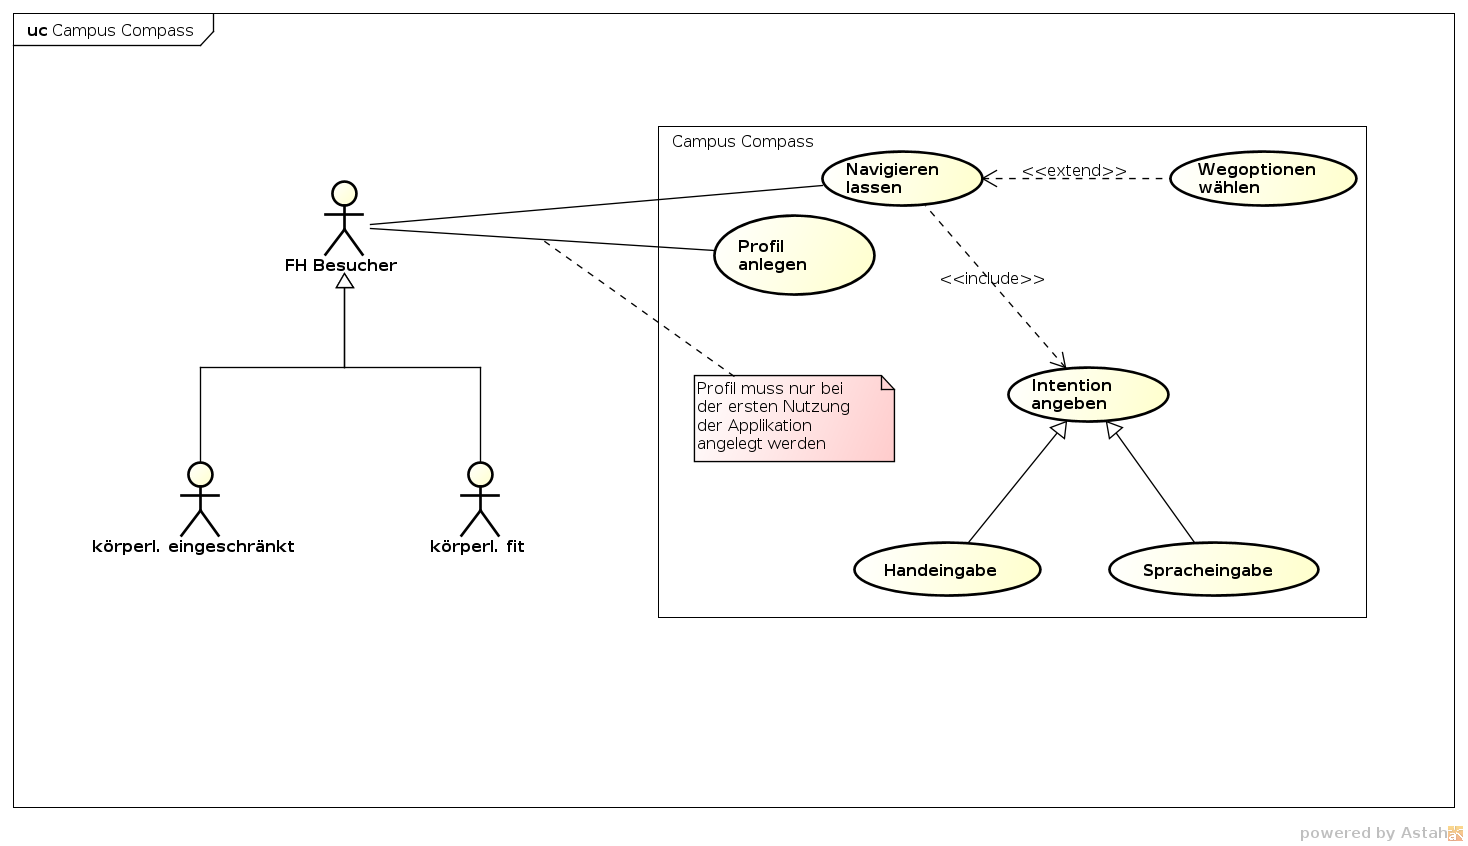
\includegraphics[width=\linewidth]{img/use-case-diagram.png}
  \label{img:use-case-diagramm}
  \caption{Use Case Diagramm}
\end{figure}

\noindent Es fällt auf, dass der Nutzer nur einen\footnote{Das Pflegen des Profils geschieht höchstwahrscheinlich nur bei der ersten Nutzung der Applikation} echten Use Case hat: \emph{Navigieren lassen}. Hieraus lässt sich für das Oberflächendesign ableiten, dass der Nutzer bei der Bedienung der Applikation möglichst schnell mit der Navigation beginnen möchte und eventuelle Details lieber während der Navigation einstellen wird. 

\subsubsection*{Aktivitätsdiagramme (Verhalten)}
... bieten eine standardisierte Möglichkeit um die zuvor im Use-Case-Diagramm gezeigten Aktivitäten im Detail darzustellen. Sie zeigen die Aktionen, aus denen sich eine Aktivität zusammensetzt, sowie den Aktivitätsfluss.

\begin{figure}[hbt]
  \centering
  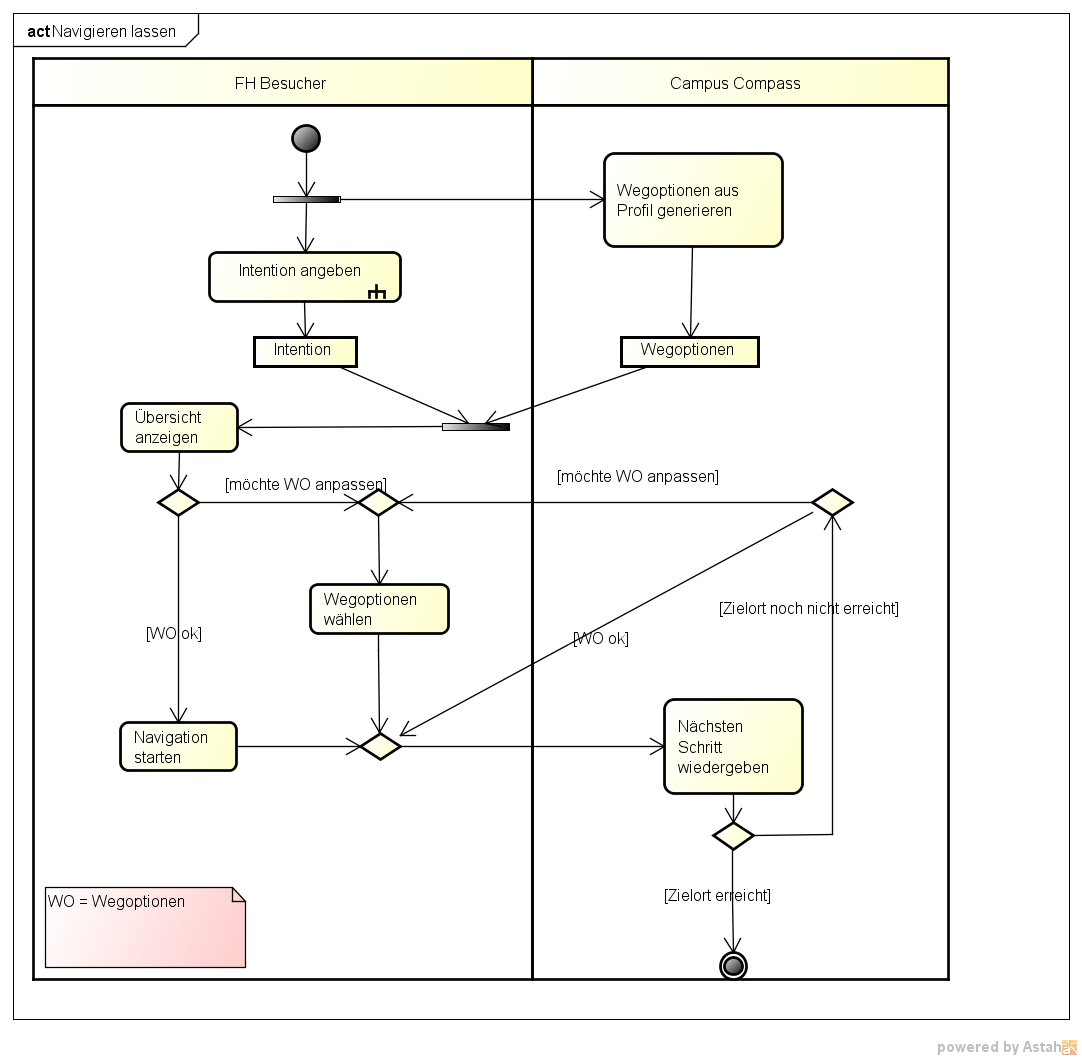
\includegraphics[width=\linewidth]{img/akt_navigieren_lassen.png}
  \label{img:akt_navigieren_lassen}
  \caption{Navigieren lassen}
\end{figure}

Das Use Case Diagramm \emph{Navigieren lassen} zeigt anschaulich den Verlauf einer Wegführung. Nach dem der FH Besucher seine Intention der App mitgeteilt hat, bekommt er eine Übersicht seiner Auswahl angezeigt. Nun beginnt ein Kreislauf, in dem der Anwender während der gesamten Wegführung die Möglichkeit hat Wegoptionen anzupassen, während die erforderlichen Schritte um das Ziel zu erreichen nacheinander aufgeführt werden. Gibt es keinen weiteren Schritt mehr, ist der Zielort erreicht.

\begin{figure}[hbt]
  \centering
  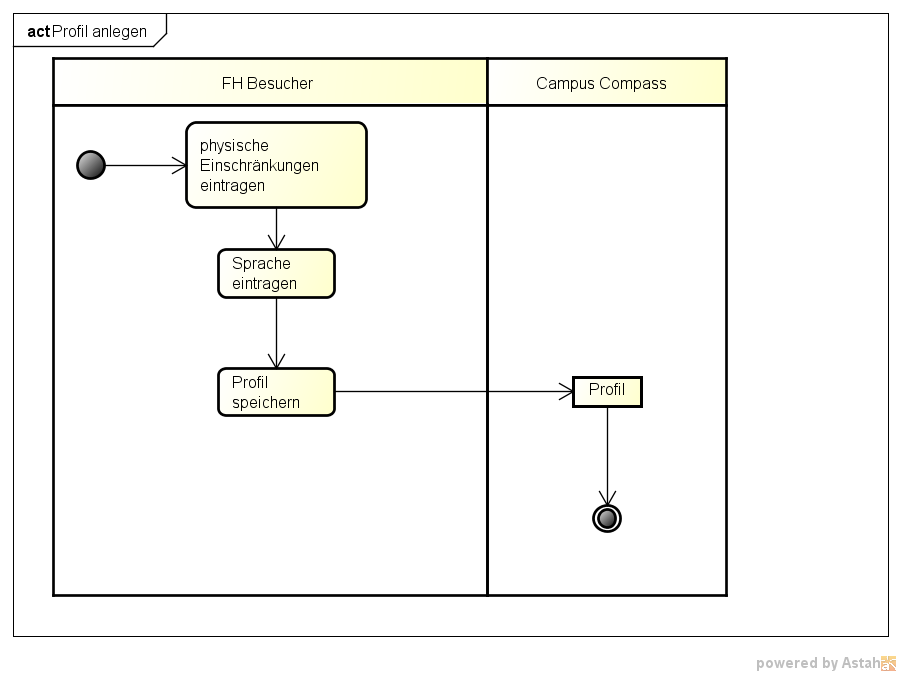
\includegraphics[width=\linewidth]{img/akt_profil_anlegen.png}
  \label{img:akt_profil_anlegen}
  \caption{Profil anlegen}
\end{figure}
